\documentclass[a4paper,10pt]{article}\usepackage[]{graphicx}\usepackage[]{color}
%% maxwidth is the original width if it is less than linewidth
%% otherwise use linewidth (to make sure the graphics do not exceed the margin)
\makeatletter
\def\maxwidth{ %
  \ifdim\Gin@nat@width>\linewidth
    \linewidth
  \else
    \Gin@nat@width
  \fi
}
\makeatother

\definecolor{fgcolor}{rgb}{0.345, 0.345, 0.345}
\newcommand{\hlnum}[1]{\textcolor[rgb]{0.686,0.059,0.569}{#1}}%
\newcommand{\hlstr}[1]{\textcolor[rgb]{0.192,0.494,0.8}{#1}}%
\newcommand{\hlcom}[1]{\textcolor[rgb]{0.678,0.584,0.686}{\textit{#1}}}%
\newcommand{\hlopt}[1]{\textcolor[rgb]{0,0,0}{#1}}%
\newcommand{\hlstd}[1]{\textcolor[rgb]{0.345,0.345,0.345}{#1}}%
\newcommand{\hlkwa}[1]{\textcolor[rgb]{0.161,0.373,0.58}{\textbf{#1}}}%
\newcommand{\hlkwb}[1]{\textcolor[rgb]{0.69,0.353,0.396}{#1}}%
\newcommand{\hlkwc}[1]{\textcolor[rgb]{0.333,0.667,0.333}{#1}}%
\newcommand{\hlkwd}[1]{\textcolor[rgb]{0.737,0.353,0.396}{\textbf{#1}}}%
\let\hlipl\hlkwb

\usepackage{framed}
\makeatletter
\newenvironment{kframe}{%
 \def\at@end@of@kframe{}%
 \ifinner\ifhmode%
  \def\at@end@of@kframe{\end{minipage}}%
  \begin{minipage}{\columnwidth}%
 \fi\fi%
 \def\FrameCommand##1{\hskip\@totalleftmargin \hskip-\fboxsep
 \colorbox{shadecolor}{##1}\hskip-\fboxsep
     % There is no \\@totalrightmargin, so:
     \hskip-\linewidth \hskip-\@totalleftmargin \hskip\columnwidth}%
 \MakeFramed {\advance\hsize-\width
   \@totalleftmargin\z@ \linewidth\hsize
   \@setminipage}}%
 {\par\unskip\endMakeFramed%
 \at@end@of@kframe}
\makeatother

\definecolor{shadecolor}{rgb}{.97, .97, .97}
\definecolor{messagecolor}{rgb}{0, 0, 0}
\definecolor{warningcolor}{rgb}{1, 0, 1}
\definecolor{errorcolor}{rgb}{1, 0, 0}
\newenvironment{knitrout}{}{} % an empty environment to be redefined in TeX

\usepackage{alltt}

\usepackage[spanish]{babel}
	\selectlanguage{spanish}
\usepackage[utf8]{inputenc}
\usepackage[T1]{fontenc}
\usepackage{mathtools}

\title{Determinantes del consumo de la gasolina: Un estudio en los Estados Unidos de América}
\author{Justo Andrés Manrique Urbina\\Pontificia Universidad Católica del Perú\thanks{e-mail:justo.manrique@pucp.pe; ja.manrique@pm.me}}
\date{13 de mayo de 2018}
\IfFileExists{upquote.sty}{\usepackage{upquote}}{}
\begin{document} 
\maketitle
\section{Resumen}
  El presente informe analiza las determinantes del consumo de gasolina en 48 estados de los Estados Unidos de América (ahora en adelante, EUA). Para ello, se aplicaron técnicas estadísticas, como la regresión lineal múltiple bajo mínimos cuadrados ordinarios, para identificar qué variables -- detalladas en la sección 2 -- impactan el consumo del mencionado combustible. A lo largo de este informe, se evaluaron los supuestos de cada regresión realizada (tales como homocedasticidad y normalidad de los errores) y se realizó un comentario respecto a cada resultado obtenido. Posteriormente, se mencionaron los próximos pasos a realizar para un posterior análisis de los datos, de cara a los objetivos del estudio.
  
  Asimismo, el presente informe tiene como objetivo evaluar lo aprendido en el curso de Modelos Lineales 1, a cargo del profesor Sergio Camiz, de la Maestría de Estadística de la Pontificia Universidad Católica del Perú.

	\subsection{Descripción del Problema}
		El gobierno de los EUA desea entender las determinantes del consumo de gasolina. Específicamente, conocer cómo los mecanismos impositivos hacia la gasolina inciden sobre el consumo de la misma. Ello con el objetivo de:
		\begin{itemize}
			\item Entender el campo de acción que tiene, a través de estos mecanismos, el gobierno para disuadir o promover el consumo de gasolina.
			\item Conocer otras variables que impactan en el consumo y ponerlas en contraste con el mecanismo impositivo, con el objetivo de identificar la importancia relativa del mecanismo frente a otras variables.
		\end{itemize}
	\subsection{Objetivo del estudio}
		 \begin{itemize}
		 	\item Establecer un modelo lineal que permita identificar las determinantes del consumo de gasolina.
		 	\item Conocer el impacto que tiene el mecanismo impositivo respecto al consumo de gasolina.
		 	\item Conocer la importancia relativa del mecanismo impositivo frente a otras variables de estudio.
		 \end{itemize}
\section{Datos}
	Las variables concernientes al informe se obtuvieron a través de la página web de la Universidad Estatal de Florida (FSU, por sus siglas en inglés), la cual contiene la base de datos aplicable a este estudio\footnote{A continuación, se detalla la URL de dónde se obtuvieron los datos: http://people.sc.fsu.edu/~jburkardt/datasets/regression/x16.txt}. De acuerdo a lo indicado en dicha página, los datos son utilizados en el libro \emph{Applied Linear Regression} de Weisberg, edición del año 1980. En la cuarta edición, publicada el año 2014, del mencionado libro se indica que dichos datos se obtuvieron de la Administración Federal de Autopistas de los EUA\footnote{Weisberg, 2014. Pág. 15.}. Dichas variables se describen en la siguiente tabla:
	
	\begin{center}
		\begin{tabular}{p{3.5cm}|c|p{3.5cm}|p{2.5cm}}
		Nombre de la variable&Código&Descripción de la variable&Tipo de variable\\
		\hline
		\hline
		Impuesto a la gasolina&A1&El impuesto asignado a la gasolina por cada estado, en términos de centavos de dólar por galón&Cuantitativa\\
		\hline
		Ingreso per cápita promedio&A2&Ingreso promedio anual en dólares per cápita en cada estado&Cuantitativa\\
		\hline
		Millas de autopista&A3&La cantidad, en millas, de autopista construida en cada estado de EUA.&Cuantitativa\\
		\hline
		Personas con licencia de conducir&A4&La proporción de personas en cada estado, respecto al total de cada uno, que cuentan con una licencia de conducir.&Cuantitativa\\
		\hline
		Consumo de gasolina&B&La cantidad, en millones de galones consumidos en determinado estado por todo el año&Cuantitativa
		\end{tabular}
	\end{center}

\subsection{Análisis preliminar de los datos}
  Con el propósito de identificar posibles limitaciones durante la aplicación de la regresión lineal múltiple bajo mínimos cuadrados ordinarios, se realizó un análisis descriptivo de las variables descritas en la sección anterior. Al respecto, se efectuó una revisión respecto a los datos contenidos en la base de datos. Ver resumen estadístico a continuación:

% Table created by stargazer v.5.2 by Marek Hlavac, Harvard University. E-mail: hlavac at fas.harvard.edu
% Date and time: Sun, May 13, 2018 - 23:40:28
\begin{table}[!htbp] \centering 
  \caption{Resumen estadístico} 
  \label{} 
\begin{tabular}{@{\extracolsep{5pt}}lccccc} 
\\[-1.8ex]\hline 
\hline \\[-1.8ex] 
Statistic & \multicolumn{1}{c}{N} & \multicolumn{1}{c}{Mean} & \multicolumn{1}{c}{St. Dev.} & \multicolumn{1}{c}{Min} & \multicolumn{1}{c}{Max} \\ 
\hline \\[-1.8ex] 
A1 & 48 & 7.668 & 0.951 & 5.000 & 10.000 \\ 
A2 & 48 & 4,241.833 & 573.624 & 3,063 & 5,342 \\ 
A3 & 48 & 5,565.417 & 3,491.507 & 431 & 17,782 \\ 
A4 & 48 & 0.570 & 0.055 & 0.451 & 0.724 \\ 
B & 48 & 576.771 & 111.886 & 344 & 968 \\ 
\hline \\[-1.8ex] 
\end{tabular} 
\end{table} 


Se aprecia que, según lo detallado en el Cuadro 1, la base de datos de la cual se basa el presente informe se compone de 48 observaciones (cada una correspondiente a un estado de los EUA) y que los valores contenidos tienen poca variabilidad, con excepción de la variable <<Millas de Autopista>> (codificada como A3), puesto que ésta tiene una razón de desviación estándar a media alta. 

Posteriormente, se realizó un análisis gráfico de la información a fin de confirmar lo indicado en el Cuadro 2. Ver el análisis a continuación:


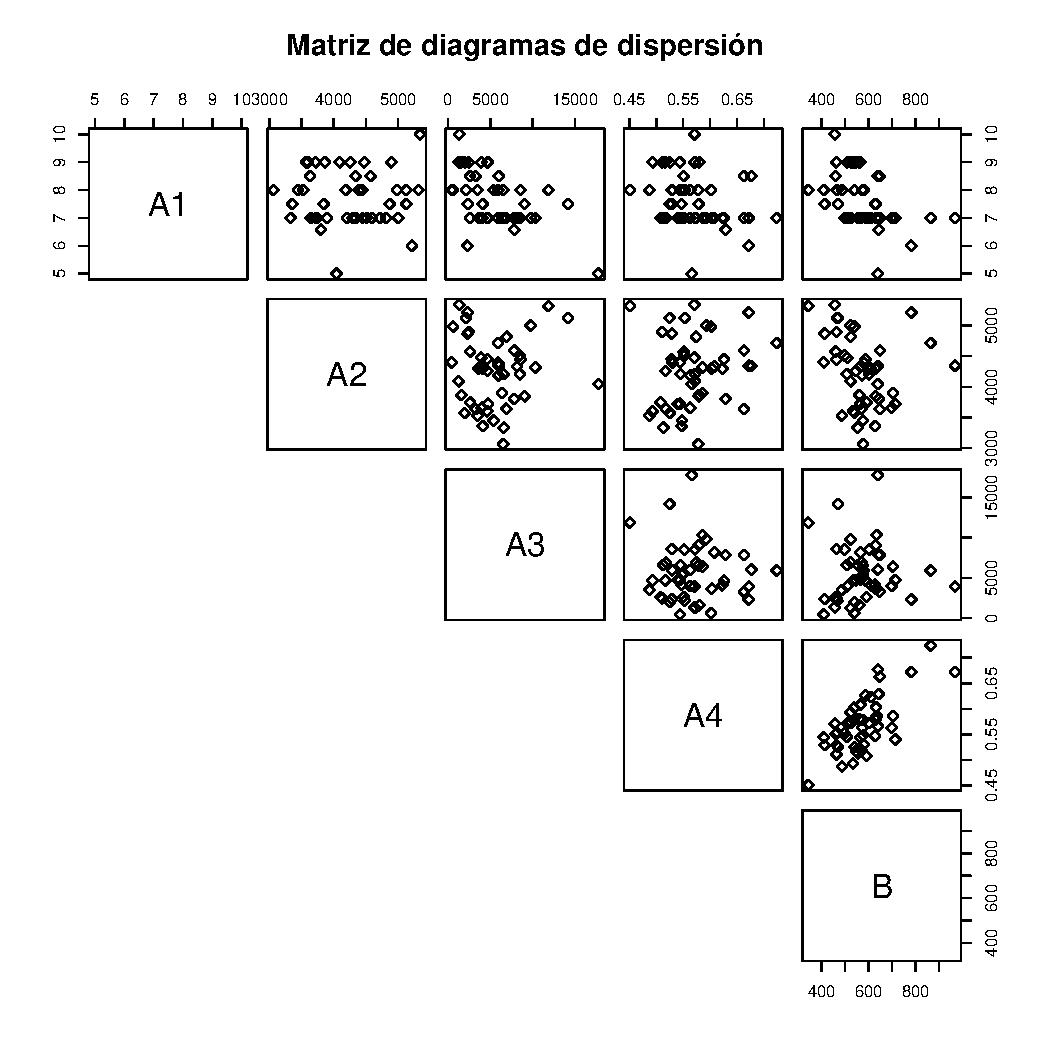
\includegraphics[width=\maxwidth]{figure/unnamed-chunk-2-1} 


Se aprecia que, según lo indicado en el cuadro precedente, existen posibles relaciones lineales en los datos los cuales se detallan a continuación\footnote{La lista comprende el análisis de los gráficos y una explicación plausible de las relaciones encontradas, sin embargo esto último comprende a un razonamiento del autor y no a un análisis estricto de datos.}:

\begin{itemize}
  \item La variable <<Impuesto a la Gasolina>> mantiene cierta relación negativa con la variable <<Millas de Autopista>>. Esto podría deberse a que, dado que los autos basados en este combustible tienen mayor millaje por recorrer, el gobierno de los EUA reducen el impuesto para no afectar económicamente a las personas.
  \item La variable <<Consumo de Gasolina>> mantiene una relación positiva con la variable <<Personas con licencia de Conducir>>. Esto podría deberse a que las personas que cuenten con licencia de Conducir mantienen autos o vehículos cuya fuente de energía es el combustible.
  \item La variable <<Consumo de Gasolina>> mantiene una relación negativa con las variables <<Impuesto a la Gasolina>> e <<Ingreso per cápita promedio>>. La primera relación podría deberse a que el impuesto tiene un carácter disuasivo respecto al consumo de la gasolina; el segundo podría deberse a que un mayor ingreso per cápita permite a las personas un mayor nivel de consumo en general.
\end{itemize}

Por último, se realizó una matriz de correlación entre las variables contenidas en la base de datos, con el fin de conocer el grado de relación que cada variable tiene respecto a las restantes. Conforme se verá en la sección 3, las variables con el prefijo <<A>> constituyen las variables predictoras y la variable <<B>> es la variable respuesta. En base a ello, el análisis de correlaciones actual está enfocado en las variables predictoras a fin de identificar \emph{a priori} los grados de colinealidad que tendrán éstas y el impacto que ello tendrá sobre la regresión lineal múltiple. Ver cuadro a continuación:


% Table created by stargazer v.5.2 by Marek Hlavac, Harvard University. E-mail: hlavac at fas.harvard.edu
% Date and time: Sun, May 13, 2018 - 23:40:33
\begin{table}[!htbp] \centering 
  \caption{Matriz de correlaciones} 
  \label{} 
\begin{tabular}{@{\extracolsep{5pt}} cccccc} 
\\[-1.8ex]\hline 
\hline \\[-1.8ex] 
 & A1 & A2 & A3 & A4 & B \\ 
\hline \\[-1.8ex] 
A1 & $1$ & $0.013$ & $$-$0.522$ & $$-$0.288$ & $$-$0.451$ \\ 
A2 & $0.013$ & $1$ & $0.050$ & $0.157$ & $$-$0.245$ \\ 
A3 & $$-$0.522$ & $0.050$ & $1$ & $$-$0.064$ & $0.019$ \\ 
A4 & $$-$0.288$ & $0.157$ & $$-$0.064$ & $1$ & $0.699$ \\ 
B & $$-$0.451$ & $$-$0.245$ & $0.019$ & $0.699$ & $1$ \\ 
\hline \\[-1.8ex] 
\end{tabular} 
\end{table} 


Se observa, según lo detallado en el Cuadro 2, que la variable <<Millas de autopista>> tiene una correlación negativa moderada (mayor a -0.5) con la variable <<Impuesto a la Gasolina>> (codificada como A1), con lo cual podría existir un problema de colinealidad en la regresión lineal múltiple. En segundo lugar, se observa que existe una correlación negativa leve entre las variables <<Impuesto a la Gasolina>> y <<Personas con licencia de conducir>> (codificada como A4). \emph{A priori} esto podría indicar que podría haber problemas de colinealidad en la regresión lineal múltiple. Sin embargo, conforme se verá en la Sección 4, la colinealidad de variables predictoras se evaluarán a través del test de inflación de varianza, en la medida estas variables formen parte del modelo final.

\section{Modelo estadístico aplicado a los datos}

Se aplicó una regresión lineal múltiple bajo mínimos cuadrados ordinarios como análisis principal de la base de datos. Al respecto, se desea modelar el consumo de la gasolina (de aquí en adelante, variable respuesta) en relación a las 4 variables restantes (de aquí en adelante, variables predictoras), de forma tal que\footnote{El modelo presentado a continuación contiene las variables codificadas. Referirse a la sección 2 para conocer el nombre de cada variable.}:

\begin{align*}
\mathrm{B}= \alpha 
    &+ \beta_{1}  \mathrm{A}_{1} \\
    &+ \beta_{2}  \mathrm{A}_{2}    \\
    &+ \beta_{3}  \mathrm{A}_{3} \\
    &+ \beta_{4}  \mathrm{A}_{4} \\
    &+ \epsilon
\end{align*}

Esta función forma el punto de partida del proceso iterativo del que se compone el presente informe. Este proceso se realiza mediante los siguientes pasos:
\begin{enumerate}
  \item Realizar una regresión lineal múltiple utilizando toda la base de datos, teniendo con variable respuesta a <<B>>, y como predictoras a las 4 restantes.
  \item Evaluar si, en su conjunto, el modelo de regresión lineal múltiple es significativo a través del estadístico F.
  \item Evaluar, a nivel individual, si las variables predictoras tienen significancia estadística y descartar aquellas insignificantes.
  \item Ejecutar una regresión lineal múltiple utilizando las variables predictoras significativas y evaluar los supuestos de homocedasticidad y normalidad en los errores y multicolinealidad.
\end{enumerate}

Ver en la sección siguiente el análisis de datos.

\section{Resultados de la regresión lineal múltiple}

Como punto de partida se ejecutó una regresión lineal múltiple utilizando todas las variables disponibles de la base de datos, atendiendo los parámetros especificados en la sección 3. Los resultados de la regresión se observan en el Cuadro 3.

% Table created by stargazer v.5.2 by Marek Hlavac, Harvard University. E-mail: hlavac at fas.harvard.edu
% Date and time: Sun, May 13, 2018 - 23:40:33
\begin{table}[!htbp] \centering 
  \caption{Regresión lineal múltiple} 
  \label{} 
\begin{tabular}{@{\extracolsep{5pt}}lc} 
\\[-1.8ex]\hline 
\hline \\[-1.8ex] 
 & \multicolumn{1}{c}{\textit{Dependent variable:}} \\ 
\cline{2-2} 
\\[-1.8ex] & B \\ 
\hline \\[-1.8ex] 
 A1 & $-$34.790$^{**}$ \\ 
  & (12.970) \\ 
  & \\ 
 A2 & $-$0.067$^{***}$ \\ 
  & (0.017) \\ 
  & \\ 
 A3 & $-$0.002 \\ 
  & (0.003) \\ 
  & \\ 
 A4 & 1,336.449$^{***}$ \\ 
  & (192.298) \\ 
  & \\ 
 Constant & 377.291$^{**}$ \\ 
  & (185.541) \\ 
  & \\ 
\hline \\[-1.8ex] 
Observations & 48 \\ 
R$^{2}$ & 0.679 \\ 
Adjusted R$^{2}$ & 0.649 \\ 
Residual Std. Error & 66.306 (df = 43) \\ 
F Statistic & 22.706$^{***}$ (df = 4; 43) \\ 
\hline 
\hline \\[-1.8ex] 
\textit{Note:}  & \multicolumn{1}{r}{$^{*}$p$<$0.1; $^{**}$p$<$0.05; $^{***}$p$<$0.01} \\ 
\end{tabular} 
\end{table} 


Del mencionado cuadro, se observa que:
\begin{itemize}
  \item El modelo, en su conjunto, tiene significancia estadística (el estadístico F tiene un p-valor menor a 0.01). Esto indica que sí existe una relación, sea lineal o no -- esto se observará a través de otros tests --, entre la variable respuesta y las predictoras.
  \item A nivel individual, la variable A3, <<Millas de autopista>> no es significativa para la variable respuesta, por lo que se procederá a descartarse.
\end{itemize}

En base a esta prueba, se realizó una nueva regresión lineal: esta vez sin considerar la variable A3. El resultado de esta regresión, la cual se compara con la regresión anterior, se observa en el Cuadro 4.


% Table created by stargazer v.5.2 by Marek Hlavac, Harvard University. E-mail: hlavac at fas.harvard.edu
% Date and time: Sun, May 13, 2018 - 23:40:33
\begin{table}[!htbp] \centering 
  \caption{Comparación entre regresiones lineales múltiples} 
  \label{} 
\begin{tabular}{@{\extracolsep{5pt}}lcc} 
\\[-1.8ex]\hline 
\hline \\[-1.8ex] 
 & \multicolumn{2}{c}{\textit{Dependent variable:}} \\ 
\cline{2-3} 
\\[-1.8ex] & \multicolumn{2}{c}{B} \\ 
\\[-1.8ex] & (1) & (2)\\ 
\hline \\[-1.8ex] 
 A1 & $-$34.790$^{**}$ & $-$29.484$^{***}$ \\ 
  & (12.970) & (10.584) \\ 
  A2 & $-$0.067$^{***}$ & $-$0.068$^{***}$ \\ 
  & (0.017) & (0.017) \\ 
  A3 & $-$0.002 &  \\ 
  & (0.003) &  \\ 
  A4 & 1,336.449$^{***}$ & 1,374.768$^{***}$ \\ 
  & (192.298) & (183.670) \\ 
  Constant & 377.291$^{**}$ & 307.328$^{*}$ \\ 
  & (185.541) & (156.831) \\ 
 \hline \\[-1.8ex] 
Observations & 48 & 48 \\ 
R$^{2}$ & 0.679 & 0.675 \\ 
Adjusted R$^{2}$ & 0.649 & 0.653 \\ 
Residual Std. Error & 66.306 (df = 43) & 65.938 (df = 44) \\ 
F Statistic & 22.706$^{***}$ (df = 4; 43) & 30.442$^{***}$ (df = 3; 44) \\ 
\hline 
\hline \\[-1.8ex] 
\textit{Note:}  & \multicolumn{2}{r}{$^{*}$p$<$0.1; $^{**}$p$<$0.05; $^{***}$p$<$0.01} \\ 
\end{tabular} 
\end{table} 


Se observa en el Cuadro 4 que:
\begin{itemize}
  \item Tanto el modelo, en su conjunto, como las variables predictoras a nivel individual son significantes (su p-valor es menor a 0.05).
  \item El R\textsuperscript{2} ajustado ha aumentado levemente en el modelo posterior, puesto que se ha descartado una variable no significativa en el análisis. Se observa que el 65.3% de la variación de la variable respuesta es explicada por las variables predictoras en el segundo modelo.
  \item El parámetro asociado a la variable A1 ha disminuido en relación al primer modelo. Esto se debe a que el grado de colinealidad con la variable descartada influyó sobre la estimación de dicho parámetro.

\end{itemize}

  Por otro lado, se computó el criterio de información de Akaike (AIC por sus siglas en inglés) para ambas regresiones. Al respecto, se observó que el AIC de la segunda regresión es levemente menor que la primera (el valor de AIC de la primera regresión es de 545.58, mientras que el de la segunda es de 544.15), por lo que el segundo modelo es de mejor calidad.
  
En base a este segundo modelo, se realizó el análisis de supuestos de la regresión lineal múltiple mediante mínimos cuadrados ordinarios. Específicamente, se efectuó el análisis de:

\begin{itemize}
  \item Homocedasticidad y normalidad de los errores.
  \item Multicolinealidad de las variables predictoras.
\end{itemize}

Para ello, se realizó el diagnóstico de mediante los siguientes cuadros:


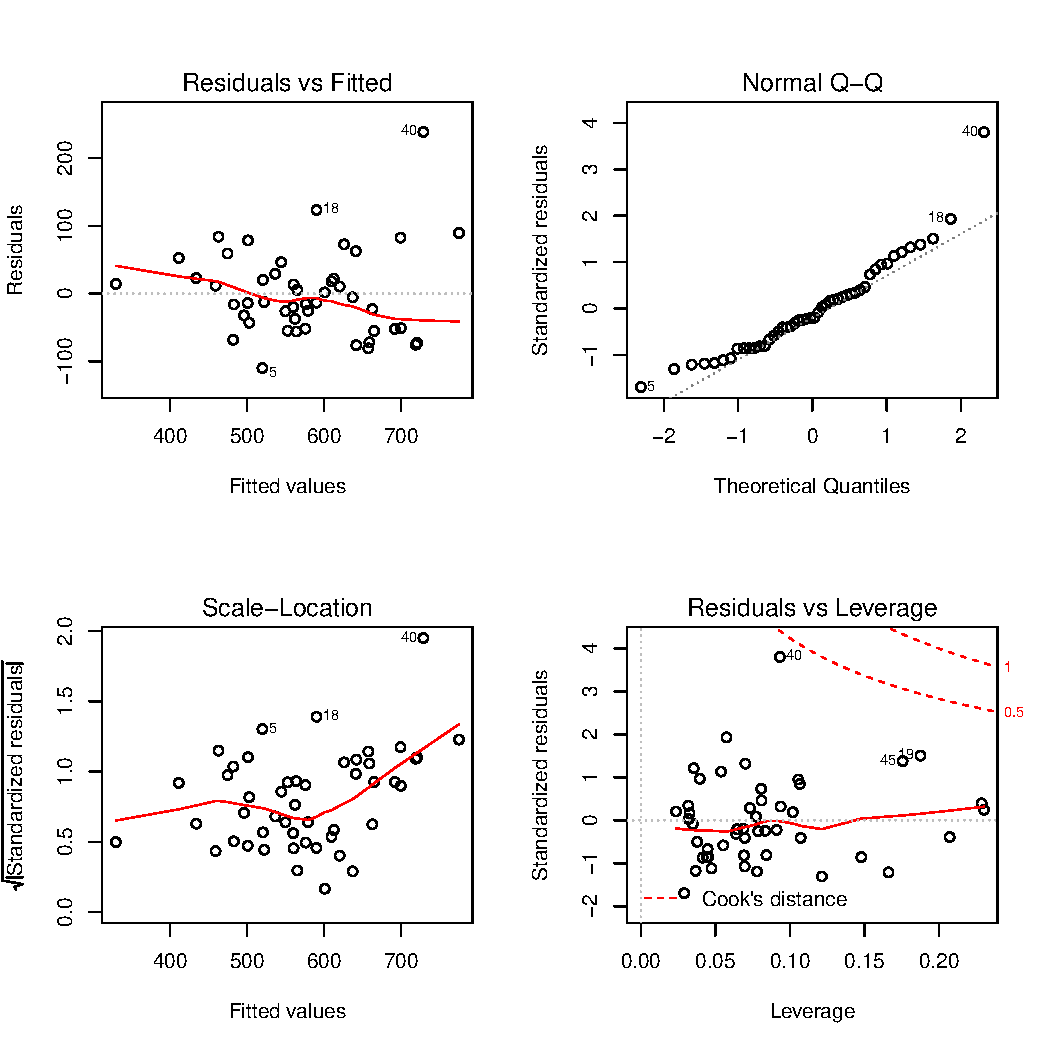
\includegraphics[width=\maxwidth]{figure/unnamed-chunk-6-1} 


En base al diagnóstico de residuos, se observa que:
\begin{itemize}
  \item La gráfica "Residuals vs Fitted" tiene como objetivo identificar si los residuales tienen un comportamiento no lineal. En esta, no se observa una relación no lineal entre los residuales; por lo tanto, se puede inferir no existe una relación no lineal que habría que modelar.
  \item La gráfica "Normal Q-Q" permite identificar si los residuos están normalmente distribuidos. En el caso los residuos no sigan, en general, una línea recta, sería un indicador que los errores no están distribuidos normalmente. En base al cuadro presentado, se podría concluir que los errores tienen una distribución normal\footnote{Esto será puesto a prueba con la prueba Shapiro-Wilks.}.
  \item La gráfica "Scale-Location" permite identificar si los errores son homocedásticos o no. En ese sentido, si hubiere algún grado de linealidad en esta gráfica, ello implicaría que los errores no tienen varianza constante por lo que no serían homocedásticos. En base al cuadro presentado, un grado de linealidad en la medida que el valor predicho aumenta; por lo tanto, se podría concluir que los errores son heterocedásticos\footnote{Esto será puesto a prueba con el comando ncvTest en R.}
  \item La gráfica "Residuals vs Leverage" permite identificar puntos aberrantes dentro de la base de datos. En base al cuadro presentado, las observaciones N° 40, 19 y 45 tienen una distancia de Cooks mayor que las otras observaciones. Sin embargo, no superan los umbrales como para tener un impacto significativo.
\end{itemize}

Finalmente, se efectuaron tests estadísticos de homocedasticidad y normalidad de los errores a fin de validar los supuestos de la regresión lineal múltiple bajo mínimos cuadrados ordinarios. Ver resultados a continuación:

\begin{itemize}
  \item Prueba de Normalidad de Errores (Shapiro-Wilks)
    \begin{itemize}
      \item El test de Shapiro-Wilks está orientado a identificar si los errores siguen una distribución normal, a fin de validar los supuestos de la regresión. La hipótesis nula de dicho test es que una determinada muestra proviene de una población normalmente distribuida (Camiz, 2018). Conforme se aprecia en el cuadro posterior, el p-valor del test es menor a 0.05 por lo que se rechaza dicha hipótesis nula. Por lo tanto, los residuos no siguen una distribución normal.
\begin{knitrout}
\definecolor{shadecolor}{rgb}{0.969, 0.969, 0.969}\color{fgcolor}\begin{kframe}
\begin{verbatim}
## 
## 	Shapiro-Wilk normality test
## 
## data:  reg_2$residuals
## W = 0.9282, p-value = 0.005858
\end{verbatim}
\end{kframe}
\end{knitrout}
    \end{itemize}  
  \item Prueba de Homocedasticidad de Errores (Prueba de Breusch-Pagan)
    \begin{itemize}
      \item El test de Breusch-Pagan está orientado a identificar si los errores tienen una varianza homocedástica, a fin de validar los supuestos de la regresión. La hipótesis nula de dicho test es que los errores son homocedásticos (Camiz,2018). Conforme se aprecia en el cuadro posterior, el p-valor del test es menor a 0.05, por lo que se rechaza la hipótesis nula. Por lo tanto, los residuos no tienen una varianza constante (es heterocedástico).
\begin{knitrout}
\definecolor{shadecolor}{rgb}{0.969, 0.969, 0.969}\color{fgcolor}\begin{kframe}
\begin{verbatim}
## Non-constant Variance Score Test 
## Variance formula: ~ fitted.values 
## Chisquare = 11.0997    Df = 1     p = 0.0008634181
\end{verbatim}
\end{kframe}
\end{knitrout}
    \end{itemize}
\end{itemize}

\section{Discusión y conclusiones}

En base al análisis presentado, se observa que:
\begin{itemize}
  \item Respecto a la regresión lineal múltiple
      \begin{itemize}
          \item Las variables predictoras, exceptuando <<Millas de autopista>>, son parte de las determinantes del consumo de gasolina. Se puede apreciar lo siguiente, según el Cuadro 4:
              \begin{itemize}
                  \item Un incremento de un centavo por galón en el impuesto a la gasolina incide en una disminución de 29.4 millones de galones de gasolina.
                  \item Un incremento de un dólar en el ingreso per cápita de cada estado incide en una disminución de -0.068 millones de galones de gasolina.
                  \item Un incremento de un 1 por ciento de la proporción de conductores en cada estado incide en un aumento de 1,374.768 millones de galones de gasolina.
            \end{itemize}
      \end{itemize}
  \item Respecto a los supuestos de la regresión:
    \begin{itemize}
      \item Se observa que los errores son heterocedásticos y no mantienen una distribución normal, por lo que con los datos actuales no es posible tomar por válida la regresión lineal múltiple.
    \end{itemize}
\end{itemize}

En base a esta información, se propone, con el fin de superar dichas limitaciones a la regresión lineal múltiple:

\begin{itemize}
  \item Recolectar información adicional que sirva para el análisis del consumo de la gasolina, como por ejemplo:
      \begin{itemize}
          \item Proporción de autos basados en combustible.
          \item Cantidad de vehículos en circulación en cada estado.
          \item Población (en cantidad de personas) en cada estado
      \end{itemize}
  \item En caso los supuestos de una nueva regresión con información adicional no se cumplan, se sugiere entrar a un análisis por distritos y ya no por estados, a fin de obtener mayor cantidad de observaciones.

\end{itemize}

\section{Bibliografía}
Camiz, Sergio. 2018. Pontificia Universidad Católica del Perú.\emph{Notas de Clase}.

Weisberg, Sanford. 2014. Wiley. \emph{Applied Linear Regression}.

Faraway, Julian. 2015. CRC Press. \emph{Linear Models with R}.

Universidad Estatal de Florida. \emph{Regression Datasets}. URL: <<http://people.sc.fsu.edu/~jburkardt/datasets/regression/x16.txt>>. Consulta realizada: 2 de abril de 2018.

\end{document}
